\addtocontents{toc}{\newpage}
\chapter{Heuristic Search}
\label{chap5}
\section{Motivation}
As discussed in the Chapter \ref{chap3}, many complex methods have been applied to the search problem. These methods take varied approaches such as reduction to a travelling salesman problem and making use of industrial solvers \cite{P1}, variable neighbourhood search \cite{P1,P5,P7}, genetic algorithms \cite{P7,P19}, ant colony optimization \cite{P5,P19} and reformulation as an integer linear programming problem \cite{P6}.

However, at least in the first instance, we decide to focus upon relatively simple greedy heuristics. Some reasons for this decision are:
\begin{itemize}
\item The heuristics run significantly faster than the aforementioned methods. This allows for ease of prototyping and the ability to easily experiment with many variations on both the search and cost functions.
\item The inner-workings of the heuristics are transparent. This transparency allows for ease in diagnosing problems with either the heuristics themselves or with the cost functions. The transparency also allows for easy visualisation of every individual search step which enables us to observe exactly how errors occur and are how they are propagated. In contrast, using some of the previous methods would make it difficult to diagnose, for instance, whether an error is caused by the search or the cost function.
\item Any advanced search methods need to be compared against a solid baseline. These heuristics provide such a baseline.
\item Surprisingly good performance has been obtained using greedy heuristics. For instance, \cite{P2} reports that their simple heuristic search managed to outperform both a variable neighbourhood search and an ant colony optimization method.
\item The heuristics can cope with inputs containing missing shreds or extra shreds coming from different documents. This robustness is a consequence of the heuristic's bottom up formulation, which needs to make fewer assumptions than the top down optimizing solutions.
\end{itemize}

\section{Description}
\label{chap5Desc}
Despite the fact that most of the previous work has focused on complex search algorithms, a few greedy heuristics have been explored before. We first re-implement 3 of these heuristics which, in growing order of complexity, are: the \emph{Row building} heuristic \cite{P5}, the \emph{Prim based} heuristic \cite{P5} and the \emph{ReconstructShreds} heuristic \cite{P2}. More details about these techniques are available in Section \ref{chap2Search}. Additionally, we implement a fourth, novel, heuristic which is an extension of the ReconstructShreds version. 

The central idea behind the ReconstructShreds heuristic is that, at each search step, the best available edge should be added to the partial solution. A few steps of the execution of this algorithm are examined in Figure \ref{fig:kruskal}, where all groups of shreds of size 2 or larger are shown (i.e. the individual pieces, which are groups of size 1, are omitted from the figure). The algorithm will continue to add the best possible edge to the partial solution and thus enlarge and merge clusters until only 1 cluster is left. This final cluster is the algorithm's final solution. 

\begin{figure}[h]
        \centering
        \begin{subfigure}[b]{0.49\textwidth}
                \centering
                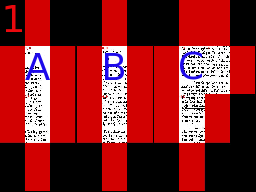
\includegraphics[width=\textwidth, height=4.5cm]{kruskal1}
                \caption{There are 3 clusters: A, B and C \vspace{2\baselineskip}.}
        \end{subfigure}
        ~ 
        \begin{subfigure}[b]{0.49\textwidth}
                \centering
                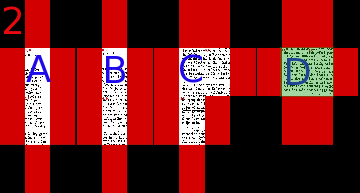
\includegraphics[width=\textwidth, height=4.5cm]{kruskal2}
                \caption{Best edge was between 2 shreds which belonged to neither cluster. Therefore a new cluster is created.}
        \end{subfigure}
        ~ 
        \begin{subfigure}[b]{0.49\textwidth}
                \centering
                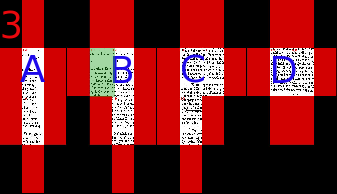
\includegraphics[width=\textwidth, height=4.5cm]{kruskal3}
                \caption{Best edge was between a shred belonging to cluster B and one belonging to neither cluster. Therefore cluster B is enlarged.}
        \end{subfigure}
        ~ 
        \begin{subfigure}[b]{0.49\textwidth}
                \centering
                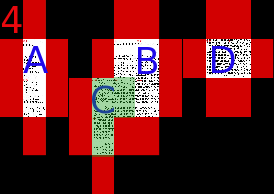
\includegraphics[width=\textwidth, height=4.5cm]{kruskal4}
                \caption{Best edge was between a shred belonging to cluster B and one belonging to cluster C. Therefore the two clusters are merged.}
        \end{subfigure}
        \caption{Four steps from the middle of a ReconstructShreds search are shown. The clusters are called A, B, C and D, the green pieces highlight the changes that occur in every step and the red pieces show the positions that are considered for the insertion of new shreds.}
        \label{fig:kruskal}
\end{figure}

\subsection{Analysis of ReconstructShreds}
This algorithm calculates all the edge probabilities and goes through the list in descending order. Whenever it encounters a valid edge, it adds it to the solution set (see Algorithm \ref{alg:RS} for the pseudocode \footnote{The pseudocode in this chapter assumes the existence of a disjoint-set data structure which can perform operations such as $InitSet(x)$ (create a set with the element $x$ in it), $GetSet(x)$ (return the set to which $x$ belongs) and various set operations such as $Union(S_x,S_y)$ and $Intersect(S_x,S_y)$}).

\begin{algorithm}[h]
\caption{The ReconstructShreds heuristic}
\begin{algorithmic}[1]
\Statex \Comment{Takes the set of edges and the set of shreds as input} 
\Procedure {ReconstructShreds}{$S_{edges}$, $S_{shreds}$} 
  \State $probs \gets []$ \Comment{Initialize 2 empty arrays for the probabilities and edges}
  \State $edges \gets []$ 
  \ForAll{$E_x \in S_{edges}$} 
    \ForAll {$E_y \in S_{edges}$}
      \State $probs[(E_x,E_y)] \gets \Pr(E_x,E_y)$ \Comment{Calculate and store all the probabilities}
    \EndFor
  \EndFor
  \Statex
  \State $setsLeft \gets |S_{shreds}|$  \Comment{Initially every shred is its own set, initialize these}
  \ForAll{$S_x \in S_{shreds}$}
    \State $InitSet(S_x)$
  \EndFor
  \Statex
  \While{$setsLeft > 1$} \Comment{Get the edges with the max probability}
    \State $(E_x,E_y) \gets \arg\max_{(E_x,E_y)} probs[(E_x,E_y)]$ 
    \State $S_x \gets GetSet(E_x)$ \Comment{Retrieve the sets of these 2 edges} 
    \State $S_y \gets GetSet(E_y)$
    \If{$S_x \neq S_y ~ \& ~ mergePossible(E_x,E_y)$} 
      \State $S_x \gets Union(S_x,S_y)$ \Comment{If the edge is valid, merge the two sets}
      \State $S_y \gets Union(S_x,S_y)$
      \State $edges.append((E_x,E_y))$
      \State $setsLeft \gets setsLeft - 1$  
    \EndIf
    \State $probs[(E_x,E_y)] \gets 0$ \Comment{make sure the processed edge isn't picked again} 
  \EndWhile
  \Statex
  \State \textbf{return} $edges$ \Comment{The set of returned edges describes a complete solution} 
\EndProcedure
\end{algorithmic}
\label{alg:RS}
\end{algorithm}

The problem with this approach is that the probabilities used are static and therefore the algorithm is completely ignorant of the formed partial solution. Its only interaction with the current state of the solution occurs via the $mergePossible(E_x,E_y)$ function which just tells the algorithm if the current solution allows for that particular merge. In particular, the algorithm takes no account of the fact that when merging 2 sets of pieces, several new edges may form. Therefore the ReconstructShreds heuristic would be happy to merge two large sets of pieces based on 1 good edge resulting from the merge even if several other terrible edges also result from that same match (see Figure \ref{fig:rsp}).

\begin{figure}[h]
    \centering
    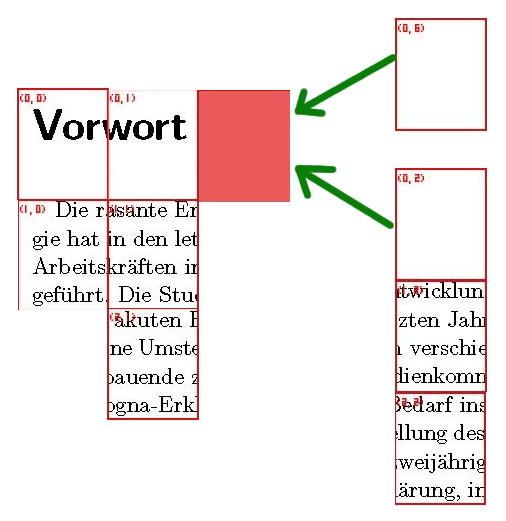
\includegraphics[width=\textwidth]{recShredProb}
    \caption{Here two potential matches for the red slot are shown. The first match is a single white piece, while the second match is a group of 3 shreds that perfectly aligns with our target shreds. Since ReconstructShreds will only look at one edge, both matches will have an identical score, namely that assigned to all white on white matches. ReconstructShreds cannot take advantage of the extra information gained since the second white shred was merged with additional shreds.}
    \label{fig:rsp}
\end{figure}

Our algorithm is designed to address this shortcoming.

\subsection[Kruskal based heuristic] {Kruskal based heuristic\footnote{This method is called a \emph{Kruskal based heuristic} because the main goal of the method, namely that of always adding the best available edge to the solution, is analogous to the goal of the minimum spanning tree algorithm, Kruskal \cite{P9}. Therefore the general Kruskal method can be extended to this specific problem, with the only additional difficulty of having to reject potential matches which would result in 2 shreds overlapping. Indeed ReconstructShreds is already an extension of the Kruskal method, though the authors of \cite{P2} do not identify it as such}} 
Our approach towards resolving the problem observed in ReconstructShreds is to recalculate the probabilities of two edges matching at every iteration. By doing so we can take into account all the additional matches that would result when the sets corresponding to the 2 edges are merged (see Algorithm \ref{alg:kruskal}). 

\begin{algorithm}[h]
\caption{The Kruskal based heuristic}
\begin{algorithmic}[1]
\Procedure {Kruskal}{$S_{edges}$, $S_{shreds}$} 
  \State $edges \gets []$ 
  \State $setsLeft \gets |S_{shreds}|$ 
  \ForAll{$S_x \in S_{shreds}$}
    \State $InitSet(S_x)$
  \EndFor
  \Statex
  \While{$setsLeft > 1$}
    \State $probs \gets []$ \Comment{Probability calculation is done for every iteration}
    \ForAll{$E_x \in S_{edges}$} 
      \ForAll {$E_y \in S_{edges}$}
        \State $probs[(E_x,E_y)] \gets getProb(E_x,E_y)$  \Comment{Helper function is called}
      \EndFor
      \State $normalize(probs, E_x, S_{edges})$ \Comment{An extra normalization step is needed}
    \EndFor
    \State $(E_x,E_y) \gets \arg\max_{(E_x,E_y)} probs[(E_x,E_y)]$
    \State $S_x \gets GetSet(E_x)$ 
    \State $S_y \gets GetSet(E_y)$
    \If{$S_x \neq S_y ~ \& ~ mergePossible(E_x,E_y)$} 
      \State $S_x \gets Union(S_x,S_y)$ 
      \State $S_y \gets Union(S_x,S_y)$
      \State $edges.append((E_x,E_y))$
      \State $setsLeft \gets setsLeft - 1$  
    \EndIf
    \State $probs[(E_x,E_y)] \gets 0$ 
  \EndWhile
  \Statex
  \State \textbf{return} $edges$ 
\EndProcedure
\end{algorithmic}
\label{alg:kruskal}
\end{algorithm}

The differences between the Kruskal and the ReconstructShreds algorithms are:
\begin{itemize}
\item The probability calculation has been moved inside the \emph{while loop}, and thus our calculated probabilities need not be static any more.
\item Rather than simply taking the pre-calculated probability $\Pr(E_x,E_y)$ as the final measure of the likelihood of a match between $E_x$ and $E_y$, the helper function $getProb(E_x,E_y)$ is now called instead. This new function checks the proposed merge and identifies all the new edges that would be formed if this merge is selected (for convenience we assume the set of edges $S_x$ has a function $S_x.neighbours()$ which returns all the pairs of edges that are neighbours under this merge). The final probability is then given by multiplying the individual probabilities for every newly created edge (see Algorithm \ref{alg:getProb}).

\begin{algorithm}[h]
\caption{The getProb helper function}
\begin{algorithmic}[1]
\Procedure {getProb}{$E_x$, $E_y$}
  \State $prob \gets 1.0$
  \State $S_x \gets GetSet(E_x)$ 
  \State $S_y \gets GetSet(E_y)$ \Comment{Get the set of the proposed match}
  \State $merged \gets Union(S_x,S_y)$ 
  \ForAll{$E_a \in S_x$} \Comment{Multiply probs of new neighbours created by the match}
    \ForAll {$E_b \in S_y$}
      \If{$ (E_a,E_b) \in merged.neighbours()$} 
      \State $prob \gets prob * \Pr(E_a,E_b)$
      \ElsIf{$ (E_b,E_a) \in merged.neighbours()$}
      \State $prob \gets prob * \Pr(E_b,E_a)$
      \EndIf
    \EndFor
  \EndFor
  \State \textbf{return} $prob$
\EndProcedure
\end{algorithmic}
\label{alg:getProb}
\end{algorithm}

\item A normalization step is added. This is necessary because, by potentially multiplying the probabilities of several edges together to get the probability of our match, the sum of all probabilities is no longer guaranteed to be 1. Formally, after the normalization step taken in the calculation of the $\Pr(E_x,E_y)$ values (see Section \ref{sect:norm}) we had the following assurance: \[\forall E_a \sum_{E_x \in S_E} \Pr(E_a,E_x) = 1 \] We would like to have the same assurance regarding $getProb(E_x,E_y)$, which is why the additional normalization step is required. As before, the normalization step takes the form: \[ normProb(E_x,E_y) = \frac{getProb(E_x,E_y)}{\sum_{E_a \in S_E} getProb(E_x,E_a)} \]
\end{itemize}


\subsection{Evaluating the heuristics}
\label{chap5Eval}
We turn to evaluating the strengths and weaknesses of the algorithms discussed above.\footnote{RBH and Prim are reviewed in Section \ref{chap2Search}.} Towards this purpose we run two sets of tests. 

Firstly, we look at the performance offered by the various search functions. This is accomplished by running all the heuristics on the same input document, using the same cost function and then comparing the number of correct edges observed in the output (see Figure \ref{fig:searchScore}). 
\begin{figure}[h]
  \centering
  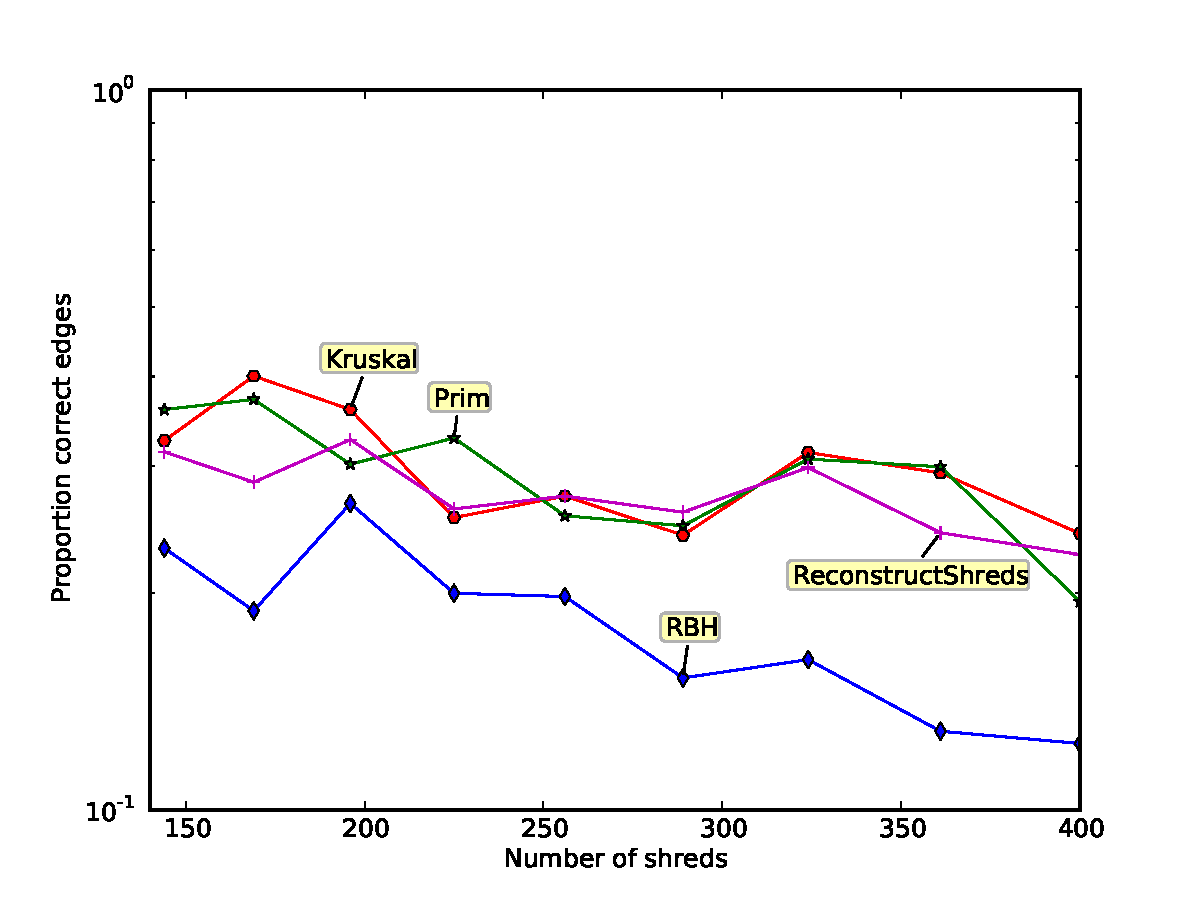
\includegraphics[width=\textwidth]{searchScores.pdf}
  \caption{The proportion of correct edges found by each search heuristic as the number of shreds increases.}
  \label{fig:searchScore}
\end{figure}
These results show that the Row Building Heuristic performs significantly worse than the others, but the performance of the top 3 heuristics is somewhat hard to compare. 

In order to try to improve upon this, a new evaluation method is proposed. This method tries to evaluate how hard it would be for a human to understand what is printed on the returned document. We therefore look at the number of moves a human would have to make to obtain the correct solution from a solution received from one of the heuristics. This assumes that the human can spot all areas of the document that are correctly reconstructed, extracts these areas and places them correctly relative to one another. Using this new evaluation method, we get Figure \ref{fig:searchGroups}, which shows that Kruskal is usually the best performing heuristic, even if not by a large margin.

\begin{figure}[h]
  \centering
  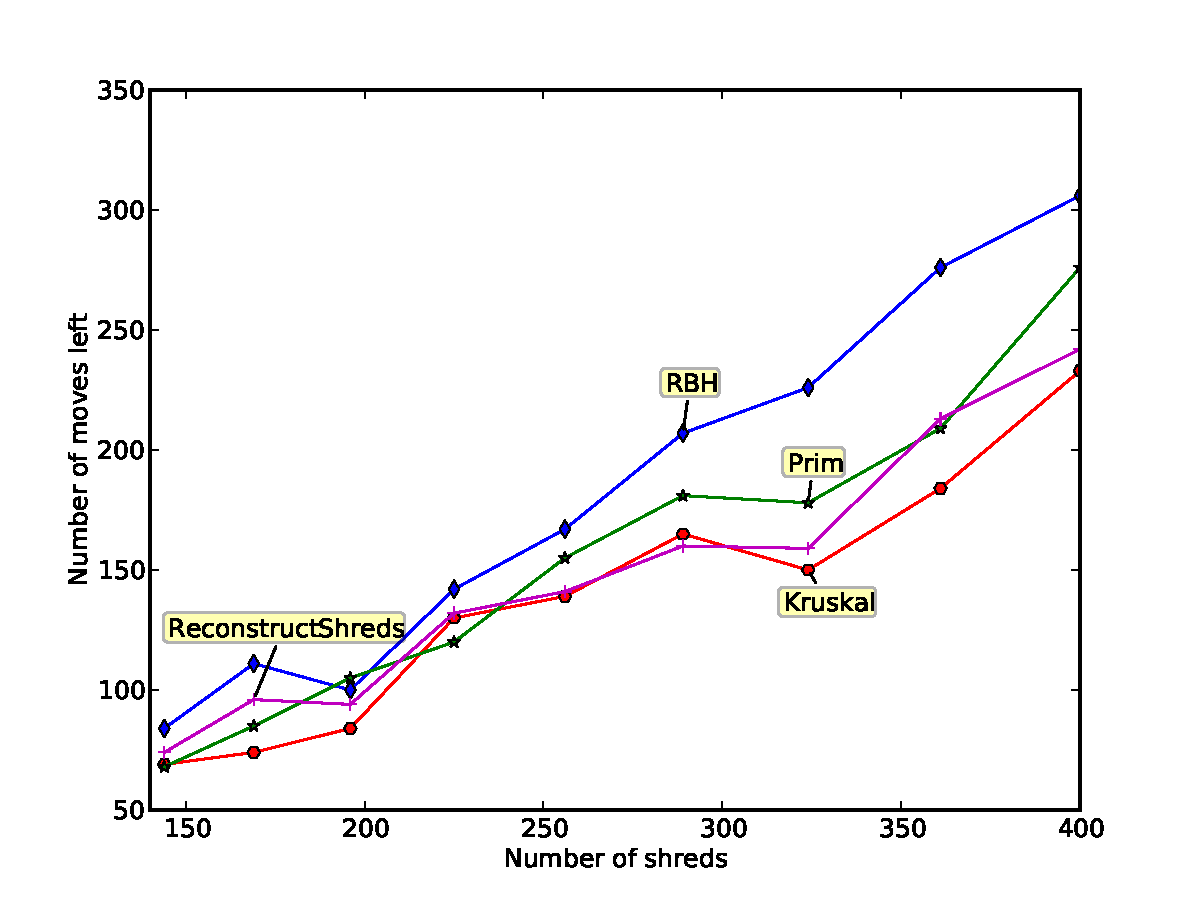
\includegraphics[width=\textwidth]{searchGroups.pdf}
  \caption{The number of moves left to perform to reach a correct solution, after running the search heuristics.}
  \label{fig:searchGroups}
\end{figure}

Secondly, we analyse the scalability of the algorithms. In real world scenarios an unshredder would potentially have to work with thousands, or even tens of thousands of pieces, which makes scalability an important factor to consider. For comparison purposes, the runtime of several more complex search functions are also shown in Figure \ref{fig:searchTime}. 
\begin{figure}[h]
  \centering
  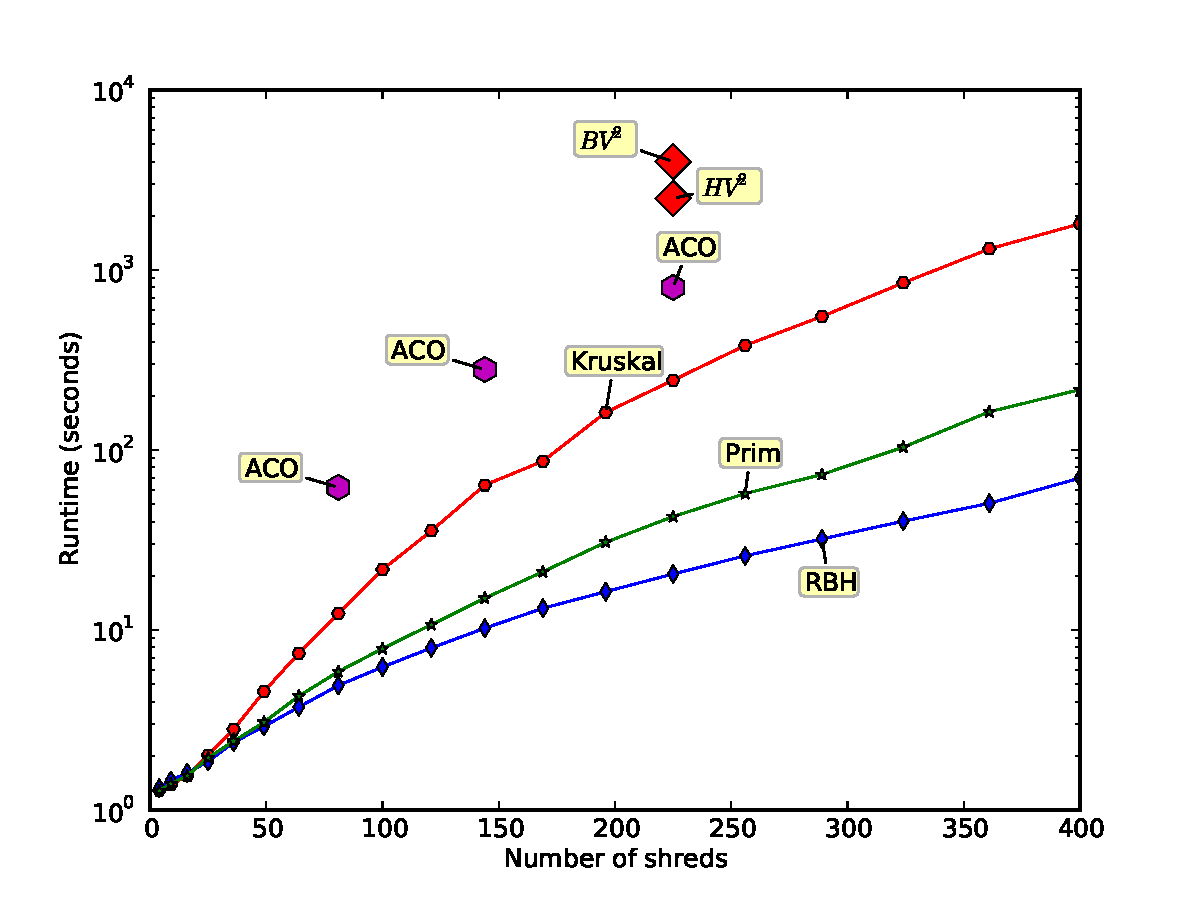
\includegraphics[width=\textwidth]{searchTime.pdf}
  \caption{Runtime comparison for 3 of the heuristics and several previously reported methods taken from \cite{P2,P5,P7}. ``ACO" is Ant Colony Optimization and ``$HV^2$" and ``$BV^2$" are two different genetic algorithms. }
  \label{fig:searchTime}
\end{figure}

As can be seen. even though the heuristics were not implemented with speed in mind\footnote{The heuristics are written in python, while the quoted optimization methods are written in C. Additionally, the implementation of ``Kruskal" is a proof-of-concept and has not been optimized at all. A non-naive reimplementation could bring its performance more in line to that of ``Prim".}, they are significantly faster than the top-down optimization methods.

\section{Cascading}
\label{chap5Casc}
All of the greedy methods presented thus far have in common an inability to correct errors. This makes them prone to a cascading effect through which an error made early in the search process can have a major effect on the result. Since there is no means through which to move the wrongly placed shred, the search will instead try to find additional pieces which match well with said shred, and these pieces will have a significant probability of also being wrong. 

In order to quantify the magnitude of this issue it is helpful to plot the function: $Error_{search}(x)$, where $x = Error_{cost}$. This function shows the proportion of errors that the search function commits when given a score function with a certain error rate. The results of this experiment\footnote{This experiment was run on synthetic data. We simulated a score function with a fixed error rate and gave the output of this function to the search heuristics} (see Figure \ref{fig:cascading}) are telling.

\begin{figure}[h]
  \centering
  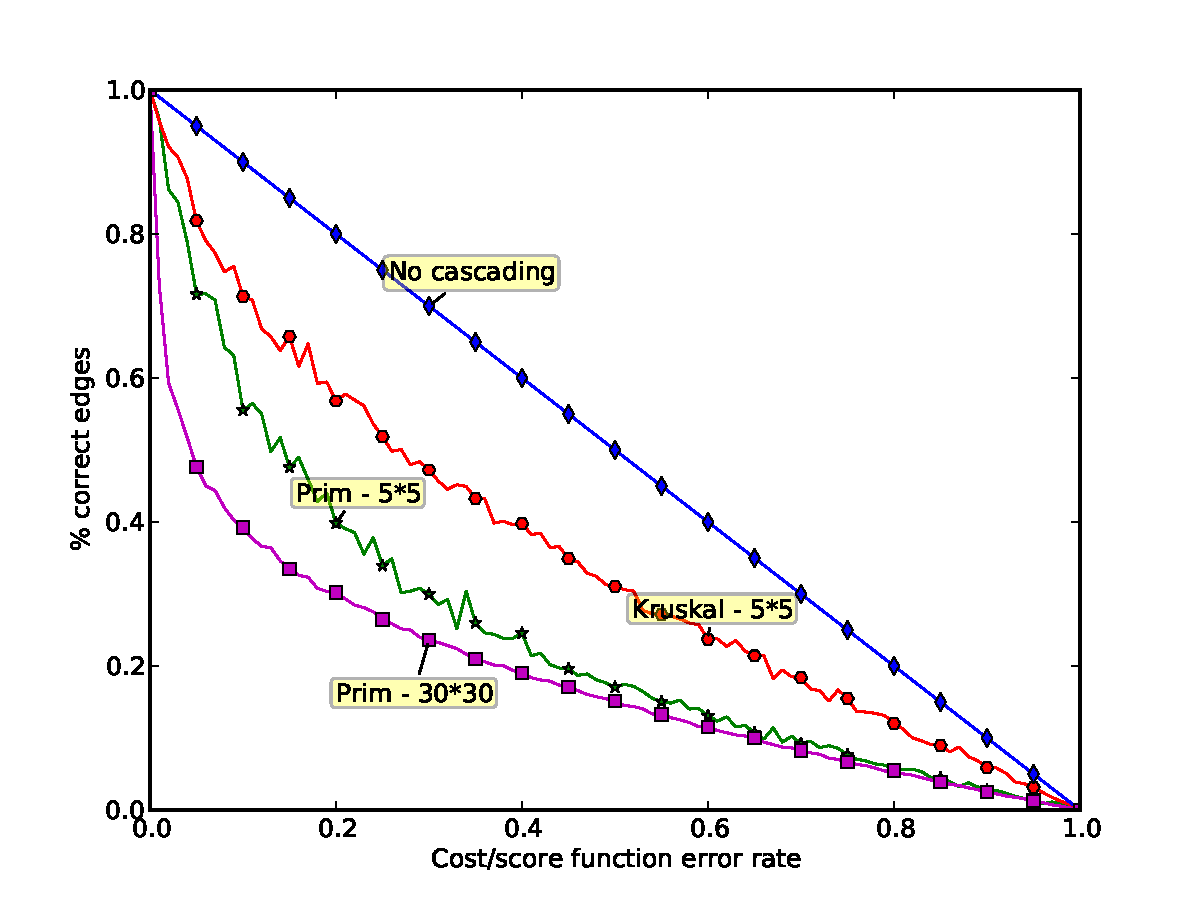
\includegraphics[width=\textwidth]{cascading.pdf}
  \caption{The effect the error in cost/score has on the final error of the method for both search heuristics on 5*5 shreds and for Prim on 30*30 shreds }
  \label{fig:cascading}
\end{figure}

Even on a tiny 5 by 5 instance, in order for the Prim heuristic to achieve 80\% accuracy the scoring function must be 95\% accurate. As can be seen, the problem only gets worse as the number of shreds increases. On a 30 by 30 instance Prim requires the same 95\% cost function accuracy rate in order to achieve a final accuracy of only 50\%.

In order to address this problem, several error correcting mechanisms were analysed. 

\newpage
\subsection{Making all shreds movable}
The simplest approach is to consider pieces that have already been placed as movable and treat them the same as the pieces which haven't been placed. Estimating the results of this formulation with the above cascading experiment gives us Figure \ref{fig:cascCorr}.

\begin{figure}[h]
  \centering
  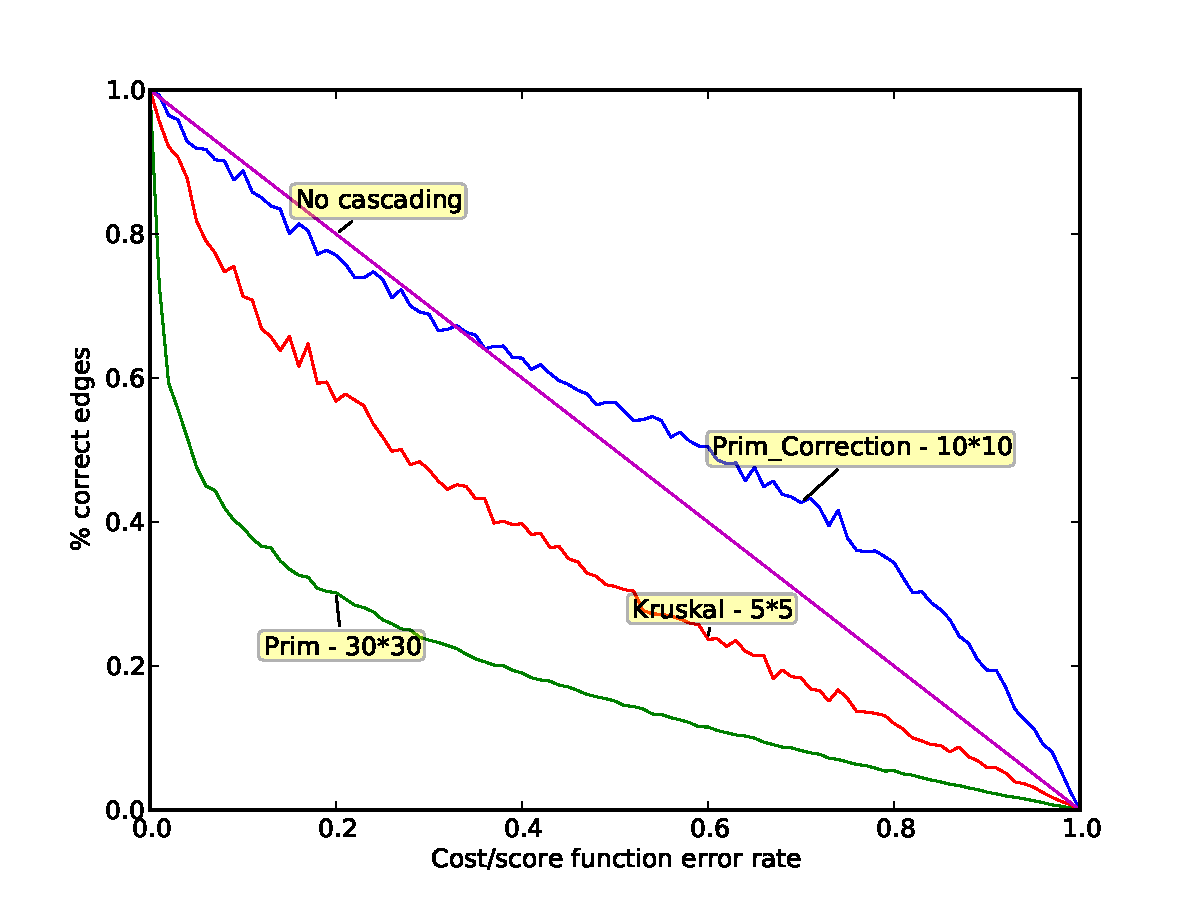
\includegraphics[width=\textwidth]{cascadingCorrection.pdf}
  \caption{Allowing already placed pieces to move ameliorates the cascading problem. Results are on 5x5 instances.}
  \label{fig:cascCorr}
\end{figure}

In theory, this approach should ameliorate the cascading problem, as we are now able to fix wrongly placed pieces. However, in practice, this basic approach can lead to an infinite cycle of moves if it happens that one piece is the best match for two different edges. In that case, the greedy algorithm will continue to switch the piece between the two different edges. This specific problem can be solved by giving the greedy correction algorithm a lookahead of size one, which ensures that a piece is only moved if the piece's score would increase. This solution however will only eliminate cycles of length 2. In order to eliminate all cycles in this way, we would require a complete examination of the search tree from the current point onwards, which quickly becomes intractable.

A different solution to the cycle problem would be to use a global score rather than a local one to determine the greedy moves. Instead of looking at the individual score of matching a shred, we could check how moving that shred affects the global score of the solution. This method indeed eliminates cycles, but introduces further problems regarding the handling of outer whitespace. If we ignore outer whitespace when calculating the global score, then we introduce an incentive for the shreds to be very dispersed as to minimize the amount of edges that count towards the score. Conversely, if we enforce outer white-space costs, we introduce a large amount of noise since most of the shreds analysed at the beginning of a solution won't end up having an external edge by the end.

We decide to stick to a local score and, in order to eliminate cycles while using a fixed size lookahead, we remember all previous states that the search has passed through and use these to detect cycles. Once a cycle is detected, we revert to the best state encountered within the cycle and then pick a move that breaks the cycle.

\subsection{Adding a post-processing step}
As mentioned above, a problem that plagues the heuristic search methods presented here is that while the search is in progress they cannot known which pieces will end up on an outer edge and which will be in the centre. This means we cannot take account of the score of an edge piece adjacent to white space, which in turn places no incentive on the search to find compact shapes that have less pieces on an outer edge.

We can ameliorate this problem by doing a post-processing step to the search. When all the pieces have been placed we finally know what the proposed outside edges are, so we can now apply a global score which keeps count of the external whitespace. Since the search we perform is still greedy, in order for the method to find correct solutions, it will require a large lookahead (see Figure \ref{fig:lookahead}). 
\begin{figure}[H]
  \centering
  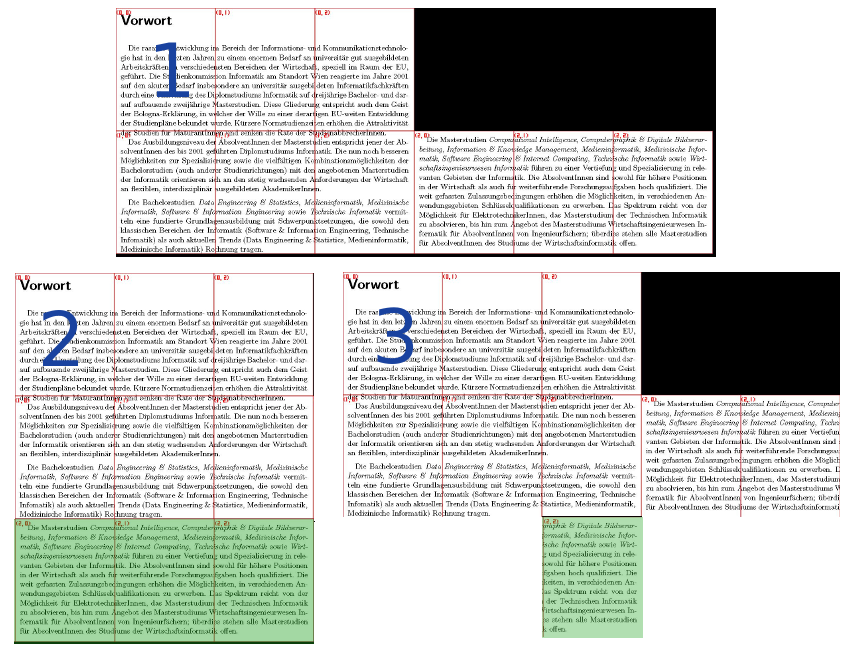
\includegraphics[width=\textwidth]{lookahead}
  \caption{In order to move from solution 1 to solution 2 the greedy search would have to pass through solution 3. However, solutions 1 and 3 both have the same number of external edges and so the same score. In this case the transition to the correct result will only be made if the search can see at least 3 moves ahead.}
  \label{fig:lookahead}
\end{figure}
As before, the lookahead requirement becomes quickly intractable. However, since all previous states are recorded, this post-processing step is guaranteed to obtain a final state that's either better or at least equivalent to the one it started with. This guarantee cannot be made for the previous correction heuristic.

\subsection{Evaluating the error-correcting methods}
Both of the above error-correcting mechanism slow down the run-time of the search significantly, as shown in Figure \ref{fig:corrScal}. The problem is that, even though infinite cycles are detected, the algorithm can still make a large number of moves before it returns to a previous state where a cycle can be stopped. Additionally, the error correcting methods make the runtime of the algorithm a lot more erratic as it ultimately depends on the nature of the encountered cycles. As can be seen in Figure \ref{fig:corrScal}, while the runtime of the original Prim algorithm increases smoothly with the number of shreds, the error correcting variants have many more peaks and valleys.
\begin{figure}[h]
  \centering
  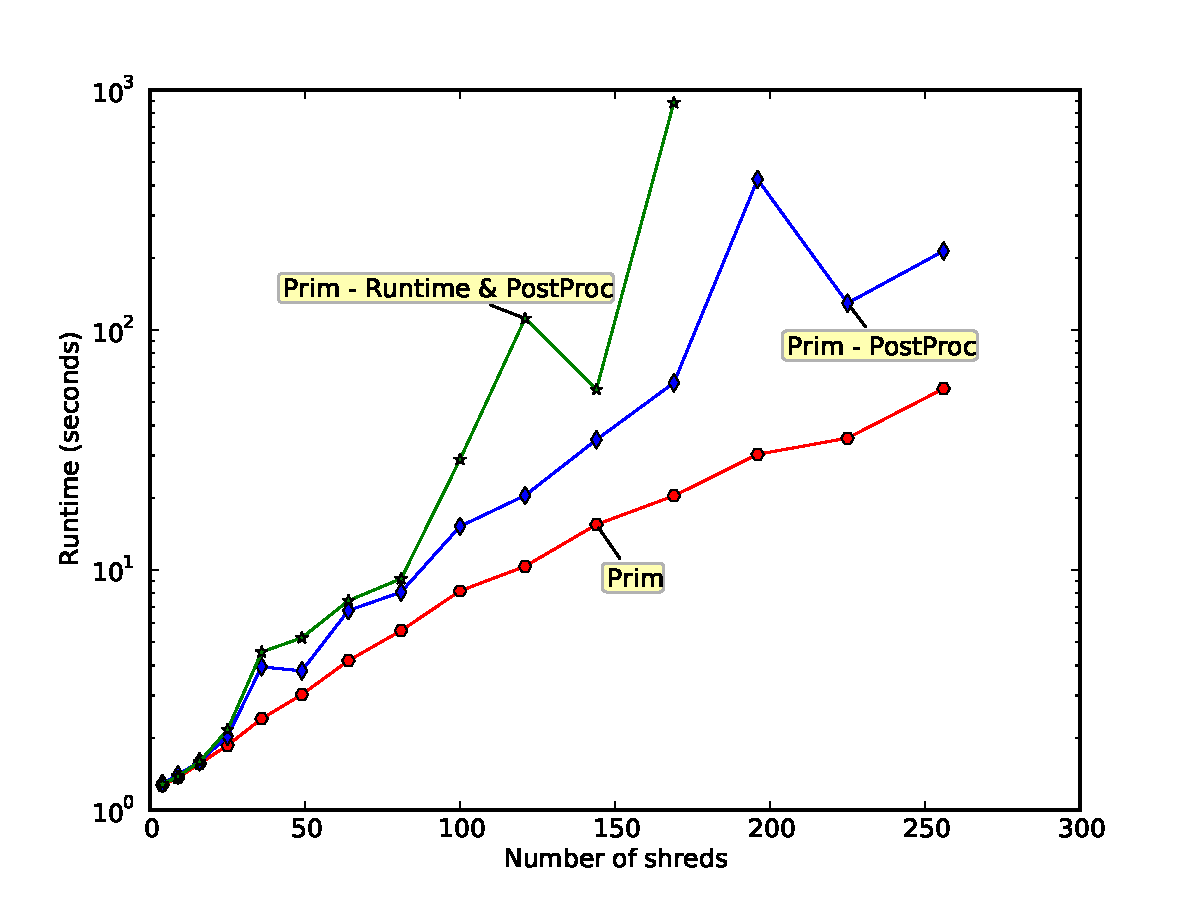
\includegraphics[width=\textwidth]{corrRuntime.pdf}
  \caption{Comparison between the basic Prim algorithm and the enhanced versions either with just the post-processing step or with both the run-time corrections and the post-processing. In the case of ``Prim - Runtime \& PostProc", the last 3 data points weren't generated as their run took longer than 20 minutes and was thus stopped.}
  \label{fig:corrScal}
\end{figure}

The performance hit shown above limits the size of the lookahead that can be used and the size of the lookahead can severely limit the performance boost obtained. With a lookahead of 1, the corrections done during the running of the search are inconsistent and may actually hurt the result. The post-processing step however provides a small but consistent boost in performance (see Figure \ref{fig:errorCorrecting})

\begin{figure}[h]
  \centering
  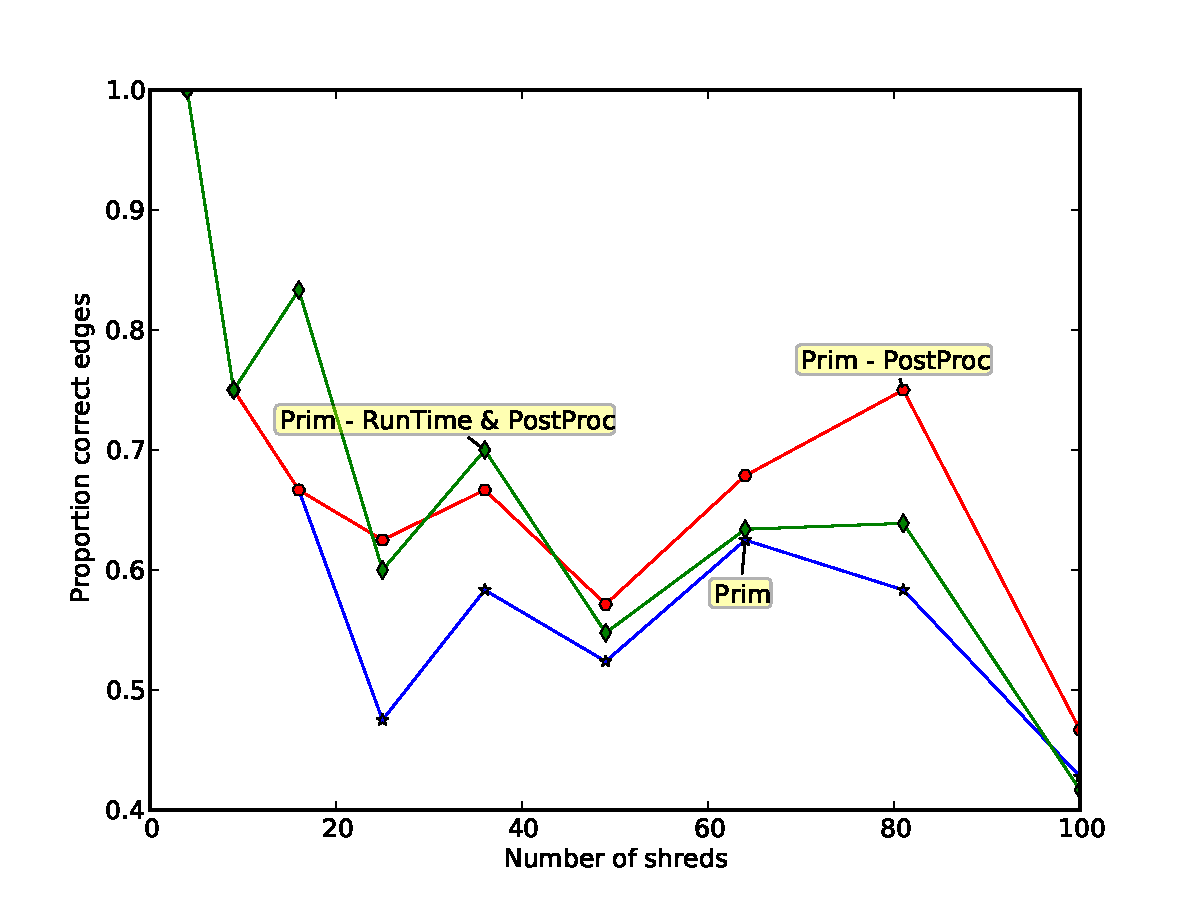
\includegraphics[width=\textwidth]{errorCorrecting.pdf}
  \caption{Comparison between the basic Prim algorithm and the enhanced versions either with just the post-processing step or with both the run-time corrections and the post-processing. The run-time corrections are not very consistent when using a small lookahead}
  \label{fig:errorCorrecting}
\end{figure}

\section{Modularity}
\label{chap5Mod}
As shown in Section \ref{chap7Rez} and throughout literature (eg: \cite{P2,P7,P34}), the reconstruction of cross-cut documents is a very difficult problem. As such, we've strived for modularity in all aspects of the proposed solution as to allow for ease of improvement and adaptation at a later time. 

The ``Kruskal" search function can also allow for modularity, by incorporating a feature called \emph{early stopping}. Since the logic behind the Kruskal method is to, at each step, pick the most likely edge, then we can intuitively return a partial solution by stopping the execution of the search when the most likely edge isn't likely enough. This allows us to use the presented search heuristic as a first step in a larger system, by reducing the search space to a dimension on which a more complex method can function. By varying the stopping condition, we can juggle a trade-off between a more aggressive reduction of the search space and an increased chance of introducing errors into the partial solution, as shown in Figure \ref{fig:stopCond}

As can be seen, even the extremely conservative \emph{99.95\%} stopping condition helps us reduce the search space to between 40\% and 80\% of its original size. Since the complexity of the search function is exponential in the number of pieces, these reductions are significant and may allow previously intractable search methods to now be run on the reduced search space. As seen from the second graph, greater reductions are possible if we can tolerate some errors in the output.
\begin{figure}[h]
        \centering
        \begin{subfigure}[b]{\textwidth}
                \centering
                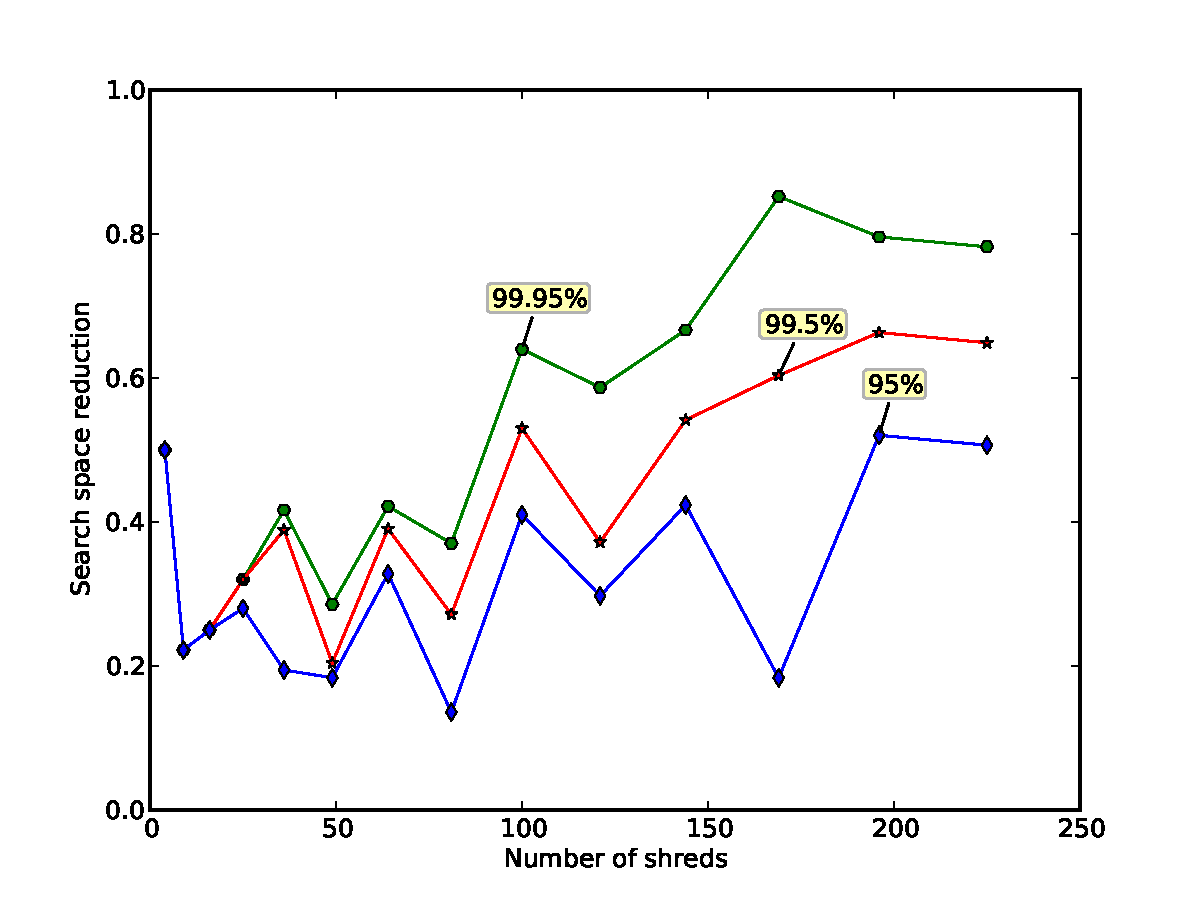
\includegraphics[width=\textwidth]{stopSearch.pdf}
                \caption{The reduction in search space corresponding to the 3 stopping conditions.  ``Search space reduction" is defined as $\frac{\mbox{Final no. pieces}}{\mbox{Initial no. pieces}}$.}
        \end{subfigure}
        ~ 
        \begin{subfigure}[b]{\textwidth}
                \centering
                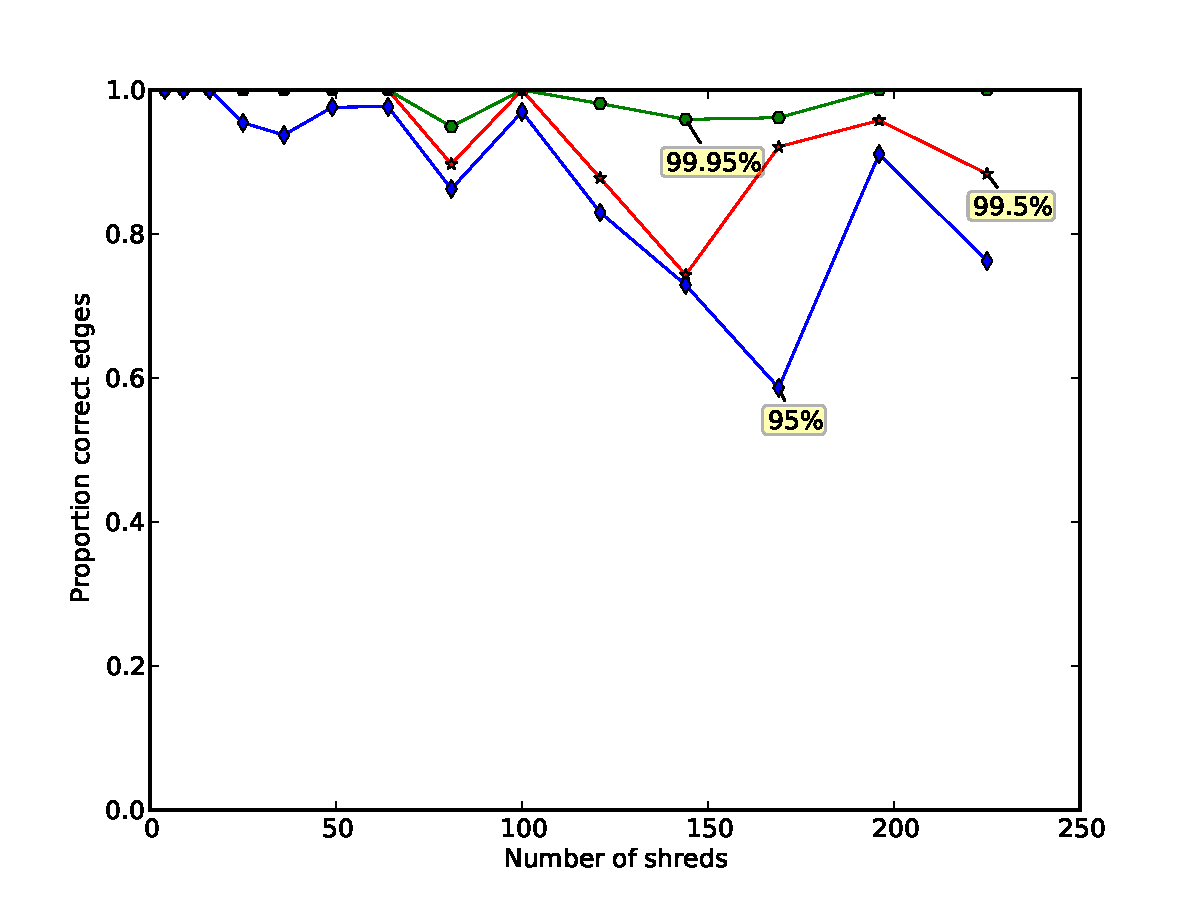
\includegraphics[width=\textwidth]{stopErr.pdf}
                \caption{The proportion of errors incurred by the 3 stopping conditions.}
        \end{subfigure}
        \caption{Trade-off between reduction in search space and errors incurred by 3 different stopping conditions.}
        \label{fig:stopCond}
\end{figure}
